%%%%%%%%%%%%%%%%%%%%%%%%%%%%%%%%%%%%%%%%%
% University Assignment Title Page 
% LaTeX Template
% Version 1.0 (27/12/12)
%
% This template has been downloaded from:
% http://www.LaTeXTemplates.com
%
% Original author:
% WikiBooks (http://en.wikibooks.org/wiki/LaTeX/Title_Creation)
%
% License:
% CC BY-NC-SA 3.0 (http://creativecommons.org/licenses/by-nc-sa/3.0/)
% 
% Instructions for using this template:
% This title page is capable of being compiled as is. This is not useful for 
% including it in another document. To do this, you have two options: 
%
% 1) Copy/paste everything between \begin{document} and \end{document} 
% starting at \begin{titlepage} and paste this into another LaTeX file where you 
% want your title page.
% OR
% 2) Remove everything outside the \begin{titlepage} and \end{titlepage} and 
% move this file to the same directory as the LaTeX file you wish to add it to. 
% Then add %%%%%%%%%%%%%%%%%%%%%%%%%%%%%%%%%%%%%%%%%
% University Assignment Title Page 
% LaTeX Template
% Version 1.0 (27/12/12)
%
% This template has been downloaded from:
% http://www.LaTeXTemplates.com
%
% Original author:
% WikiBooks (http://en.wikibooks.org/wiki/LaTeX/Title_Creation)
%
% License:
% CC BY-NC-SA 3.0 (http://creativecommons.org/licenses/by-nc-sa/3.0/)
% 
% Instructions for using this template:
% This title page is capable of being compiled as is. This is not useful for 
% including it in another document. To do this, you have two options: 
%
% 1) Copy/paste everything between \begin{document} and \end{document} 
% starting at \begin{titlepage} and paste this into another LaTeX file where you 
% want your title page.
% OR
% 2) Remove everything outside the \begin{titlepage} and \end{titlepage} and 
% move this file to the same directory as the LaTeX file you wish to add it to. 
% Then add %%%%%%%%%%%%%%%%%%%%%%%%%%%%%%%%%%%%%%%%%
% University Assignment Title Page 
% LaTeX Template
% Version 1.0 (27/12/12)
%
% This template has been downloaded from:
% http://www.LaTeXTemplates.com
%
% Original author:
% WikiBooks (http://en.wikibooks.org/wiki/LaTeX/Title_Creation)
%
% License:
% CC BY-NC-SA 3.0 (http://creativecommons.org/licenses/by-nc-sa/3.0/)
% 
% Instructions for using this template:
% This title page is capable of being compiled as is. This is not useful for 
% including it in another document. To do this, you have two options: 
%
% 1) Copy/paste everything between \begin{document} and \end{document} 
% starting at \begin{titlepage} and paste this into another LaTeX file where you 
% want your title page.
% OR
% 2) Remove everything outside the \begin{titlepage} and \end{titlepage} and 
% move this file to the same directory as the LaTeX file you wish to add it to. 
% Then add %%%%%%%%%%%%%%%%%%%%%%%%%%%%%%%%%%%%%%%%%
% University Assignment Title Page 
% LaTeX Template
% Version 1.0 (27/12/12)
%
% This template has been downloaded from:
% http://www.LaTeXTemplates.com
%
% Original author:
% WikiBooks (http://en.wikibooks.org/wiki/LaTeX/Title_Creation)
%
% License:
% CC BY-NC-SA 3.0 (http://creativecommons.org/licenses/by-nc-sa/3.0/)
% 
% Instructions for using this template:
% This title page is capable of being compiled as is. This is not useful for 
% including it in another document. To do this, you have two options: 
%
% 1) Copy/paste everything between \begin{document} and \end{document} 
% starting at \begin{titlepage} and paste this into another LaTeX file where you 
% want your title page.
% OR
% 2) Remove everything outside the \begin{titlepage} and \end{titlepage} and 
% move this file to the same directory as the LaTeX file you wish to add it to. 
% Then add \input{./title_page_1.tex} to your LaTeX file where you want your
% title page.
%
%%%%%%%%%%%%%%%%%%%%%%%%%%%%%%%%%%%%%%%%%
%\title{Title page with logo}
%----------------------------------------------------------------------------------------
%	PACKAGES AND OTHER DOCUMENT CONFIGURATIONS
%----------------------------------------------------------------------------------------

\documentclass[12pt]{article}
\usepackage[english]{babel}
\usepackage[utf8x]{inputenc}
\usepackage{amsmath}
\usepackage{graphicx}
\usepackage[colorinlistoftodos]{todonotes}

\begin{document}

\begin{titlepage}

\newcommand{\HRule}{\rule{\linewidth}{0.5mm}} % Defines a new command for the horizontal lines, change thickness here

\center % Center everything on the page
 
%----------------------------------------------------------------------------------------
%	HEADING SECTIONS
%----------------------------------------------------------------------------------------

\textsc{\LARGE Stat 427 Consulting Project}\\[1.5cm] % Name of your university/college
\textsc{\Large Terraref Prediction Metrics}\\[0.5cm] % Major heading such as course name
\textsc{\large Measures of Prediction and Ranking Accuracy for the TerraRef Project}\\[0.5cm] % Minor heading such as course title

%----------------------------------------------------------------------------------------
%	TITLE SECTION
%----------------------------------------------------------------------------------------

\HRule \\[0.4cm]
{ \huge \bfseries Title}\\[0.4cm] % Title of your document
\HRule \\[1.5cm]
 
%----------------------------------------------------------------------------------------
%	AUTHOR SECTION
%----------------------------------------------------------------------------------------



% If you don't want a supervisor, uncomment the two lines below and remove the section above
\Large \emph{Author:}\\
Kyle \textsc{Payne}\\[3cm] % Your name
Manze \textsc{Qin}\\[3cm] 

%----------------------------------------------------------------------------------------
%	DATE SECTION
%----------------------------------------------------------------------------------------

{\large \today}\\[2cm] % Date, change the \today to a set date if you want to be precise

%----------------------------------------------------------------------------------------
%	LOGO SECTION
%----------------------------------------------------------------------------------------


\includegraphics{logo.png}\\[1cm] % Include a department/university logo - this will require the graphicx package
 
%----------------------------------------------------------------------------------------

\vfill % Fill the rest of the page with whitespace

\end{titlepage}


\begin{abstract}
Your abstract.
\end{abstract}

\section{Introduction}

The following report consists of the Author's Recommendation for Measures of Prediction Quality for the TerraRef Project at the University of Illinois. In this 
preliminary report we will focus on two particular problems that have been addressed so far:

\begin{itemize}
	\item How to determine the accuracy of a continuous prediction on a continous target value (e.g. phenotype).
	\item How to Score Predicted Rankings for some subset of lines (e.g. genotypes).
\end{itemize}

While we only address these problems in a relatively closed sense, the measures that we propose may be applicable to other settings as well. We will define the our measures, describe their respective numerical and statistical properties, make recommendations for using these measures in practice, and produce functions in both the Python and R languages for their implementation. 


\section{Measures}
\label{sec:examples}

\subsection{Continuous Phenotype Prediction}

An example of the types of problems that fall under 'How to determine the accuracy of a continuous prediction on a continous target value (e.g. phenotype)' would be to demonstrate that predicted values are within 20 percent of ground truth values. Thus, we we need a measure that accounts for the difference between the predicted and ground truth (the true observed phenotype values), while also accounting for the \textit{relative degree} by which the predictions are different from the ground truth values. One metric that appears in the literature (citation) is the Relative Mean Squared Prediction Error, or the RMSPE, which we define in equation (*)

Let $Y_1, ..., Y_n$ be a set of ground truth phenotype values, and let $\hat{Y_1}, ..., \hat{Y_n}$ be the set of corresponding predictions for the ground truth phenotype values, then the RMSPE is defined as.

\begin{equation}
	RMSPE = \frac{\sqrt{\sum_{i=1}^{n}(Y_i - \hat{Y_i})^2}}{\sqrt{\sum_{i=1}^{n}Y_i^2}}}
\end{equation}

The square of the numerator $\sum_{i=1}^{n}(Y_i - \hat{Y_i})^2$ is a well-studied function within the machine learning and statistics community, known as the Mean Squared Prediction Error, or (MSPE). This is an easily computed, and numerically stable quantity that provides several desirable large sample properties. The denominator of $RMSPE$ can be viewed as the difference of the continuous ground-truth phenotype values from $0$. Thus, $RMSPE$ acts a relative measure of the difference between the ground truth continuous phenotype values, expressed in units of the continuous phenotype. Using this measure, an experimenter could make a statment such as, "I demonstrated that the predicted values are within $0.2$ of the ground truth values". This type of measure could be helpful for determining prediction accuracy for both Terminal Biomass and 3D Structural Models. Moreover, the $RMSPE$ could also be used to compare the prediction accuracy between competing models, such as comparing algorithm predictions v.s. the Lemnatec Software. 

\subsection*{Examples}

If a prediction model produces a set of predictions $\hat{Y_1}, ..., \hat{Y_n}$, for a set of ground truth continuous phenotype values $Y_1, ..., Y_n$, then 
let's state that 

\begin{equation}
	RMSPE \leq 0.20 \Rightarrow \sqrt{\sum_{i=1}^{n}(Y_i - \hat{Y_i})^2} \leq 0.2\sqrt{\sum_{i=1}^{n}Y_i^2}}
\end{equation}

The equation above describes the case where the $RMSPE$ being less than or equal to 20 percent is equivalent to stating that the mean squared prediction error is bounded by $0.2$ the size of the ground truth phenotype values. The quantity on the left-hand side of the inequality is an example of a commonly used measure of distance in mathematics, engineering, statistics, computer science, etc. known as the \textit{Norm} (Weisstein, Eric W. "Norm." From MathWorld--A Wolfram Web Resource. http://mathworld.wolfram.com/Norm.html).

Let $RMSPE_L$ be the relative mean squared prediction error of Lemnatec software predictions on the ground truth continuous phenotype values $Y_1, ..., Y_n$, which we will denote as $Y_1^{*}, ..., Y_n^{*}$. Let $RMSPE_M$ be the relative mean squared prediction error of some prediction model or algorithm. Then, making a determination such as 'algorithm predictions are no less accurate than values predicted via LemnaTec software', would require comparing $RMSPE_L$ and $RMSPE_M$, thus

\begin{equation}
	$RMSPE_M$ \leq $RMSPE_L$ 
\end{equation}

Let's assume that the predictions are for the same set of ground truth continuous phenotype values $Y_1, ..., Y_n$, then the preceding equation is 
equivalent to 

\begin{equation}
	$RMSPE_M$ \leq $RMSPE_L$ \Rightarrow \frac{\sqrt{\sum_{i=1}^{n}(Y_i - \hat{Y_i})^2}}{\sqrt{\sum_{i=1}^{n}Y_i^2}}} \leq \frac{\sqrt{\sum_{i=1}^{n}(Y_i - Y_i^{*})^2}}{\sqrt{\sum_{i=1}^{n}Y_i^2}}} \Rightarrow \sum_{i=1}^{n}(Y_i - \hat{Y_i})^2 \leq \sum_{i=1}^{n}(Y_i - Y_i^{*})^2
\end{equation}

Thus, if we compare two prediction models in $RMSPE$ on the same set of data, the comparision is equivalent to just comparing the average squared difference between the predictions and the ground truth values.
\subsection{Performance}
The Relative Mean Squared Prediction Error Performs well in situations in which there is additional noise in the continuous phenotype values $Y_1, ..., Y_n$.
For the following example, let's assume that some prediction algorithm has been fitted to a set of training data. In this case, we chose a Random Forest Model to predict Stem Biomass using the plot identifier and the precipitation data on a sub-sample of simulated data. We trained the random forest model on a sub-sample of simulated data. Predictions were then made using a test sample of the data, with additional mean $0$ gaussian random noise applied to the Stem Biomass data. The RMSPE measure increases like a polynomial with increasingly variable noise. However, the RMSPE remains relatively robust to deviations from the true Prediction Error, and only increases to very large values as the 

\begin{figure}
\centering
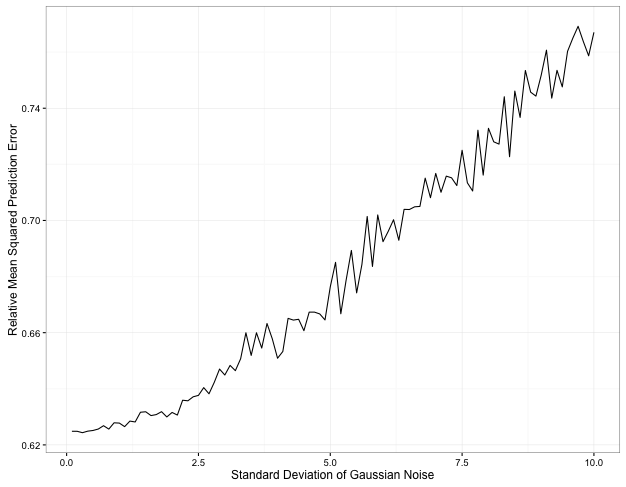
\includegraphics[width=0.75\textwidth]{robust.png}
\caption{\label{fig:robust} Robustness of RMSPE to Noise in Continuois Phenotype}
\end{figure}

\section{Ranking Scores}
Another problem of interest is assigning a score to rank predictions, e.g. given a set of lines of sorghum, and we score the predicted rank orders from some prediction algorithm? The literature is replete with measures of rank ordering. We will focus here two measures of rank ordering correlation, Kendall's Tau and the Normalized Discounted Cumulative Gain. 


\section{Kendall's Tau}

Kendall's Tau is a measure of the correlation between two sets of rankings. Let $Y_1, ..., Y_n$  be a set of observations and let $\hat{Y_1}, ..., \hat{Y_n}$ be a set of predicted observations. Then Any pair of observations $(Y_i, \hat{Y_i})$ and $(Y_j, \hat{Y_j})$, where $i \not= j$, are said to be concordant if the ranks for both elements agree: that is, if both $Y_i > Y_j$ and $\hat{Y_i} > \hat{Y_j}$ or if both $Y_i < Y_j$ and $\hat{Y_i} < \hat{Y_j}$. They are said to be discordant, if $Y_i > Y_j$ and $\hat{Y_i} < \hat{Y_j}$ and $Y_i < Y_j$ and $\hat{Y_i} < \hat{Y_j}$ . If $Y_i = Y_j$ and $\hat{Y_i} = \hat{Y_j}$, the pair is neither concordant nor discordant.

Kendall's Tau is defined as:

\begin{equation}
	\tau = \frac{(number of concordant pairs) - (number of discordant pairs)}{1/2 n(n-1)}
\end{equation}

\subsection{Tables and Figures}



\end{document}


Use the table and tabular commands for basic tables --- see Table~\ref{tab:widgets}, for example. You can upload a figure (JPEG, PNG or PDF) using the files menu. To include it in your document, use the includegraphics command as in the code for Figure~\ref{fig:frog} below.

% Commands to include a figure:
\begin{figure}
\centering
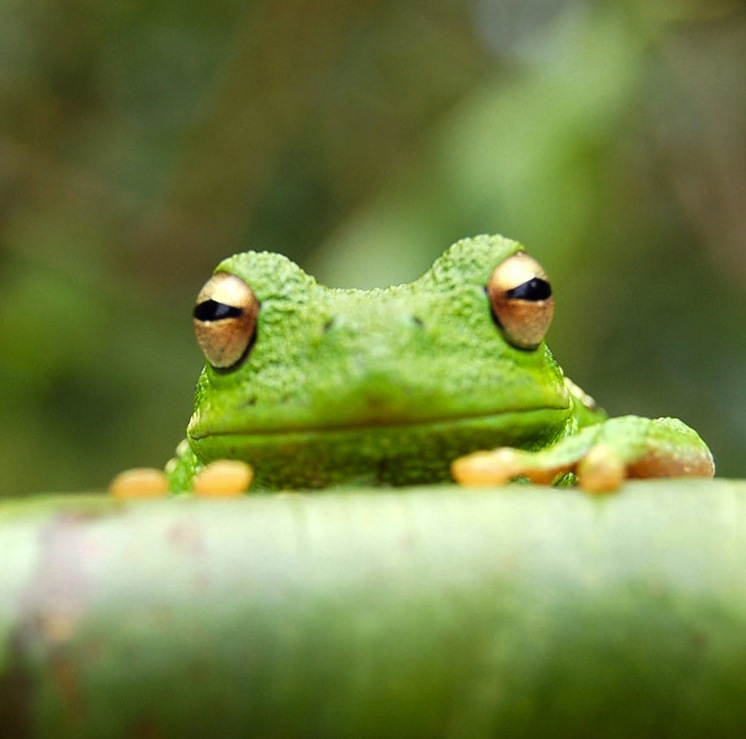
\includegraphics[width=0.5\textwidth]{frog.jpg}
\caption{\label{fig:frog}This is a figure caption.}
\end{figure}

\begin{table}
\centering
\begin{tabular}{l|r}
Item & Quantity \\\hline
Widgets & 42 \\
Gadgets & 13
\end{tabular}
\caption{\label{tab:widgets}An example table.}
\end{table} to your LaTeX file where you want your
% title page.
%
%%%%%%%%%%%%%%%%%%%%%%%%%%%%%%%%%%%%%%%%%
%\title{Title page with logo}
%----------------------------------------------------------------------------------------
%	PACKAGES AND OTHER DOCUMENT CONFIGURATIONS
%----------------------------------------------------------------------------------------

\documentclass[12pt]{article}
\usepackage[english]{babel}
\usepackage[utf8x]{inputenc}
\usepackage{amsmath}
\usepackage{graphicx}
\usepackage[colorinlistoftodos]{todonotes}

\begin{document}

\begin{titlepage}

\newcommand{\HRule}{\rule{\linewidth}{0.5mm}} % Defines a new command for the horizontal lines, change thickness here

\center % Center everything on the page
 
%----------------------------------------------------------------------------------------
%	HEADING SECTIONS
%----------------------------------------------------------------------------------------

\textsc{\LARGE Stat 427 Consulting Project}\\[1.5cm] % Name of your university/college
\textsc{\Large Terraref Prediction Metrics}\\[0.5cm] % Major heading such as course name
\textsc{\large Measures of Prediction and Ranking Accuracy for the TerraRef Project}\\[0.5cm] % Minor heading such as course title

%----------------------------------------------------------------------------------------
%	TITLE SECTION
%----------------------------------------------------------------------------------------

\HRule \\[0.4cm]
{ \huge \bfseries Title}\\[0.4cm] % Title of your document
\HRule \\[1.5cm]
 
%----------------------------------------------------------------------------------------
%	AUTHOR SECTION
%----------------------------------------------------------------------------------------



% If you don't want a supervisor, uncomment the two lines below and remove the section above
\Large \emph{Author:}\\
Kyle \textsc{Payne}\\[3cm] % Your name
Manze \textsc{Qin}\\[3cm] 

%----------------------------------------------------------------------------------------
%	DATE SECTION
%----------------------------------------------------------------------------------------

{\large \today}\\[2cm] % Date, change the \today to a set date if you want to be precise

%----------------------------------------------------------------------------------------
%	LOGO SECTION
%----------------------------------------------------------------------------------------


\includegraphics{logo.png}\\[1cm] % Include a department/university logo - this will require the graphicx package
 
%----------------------------------------------------------------------------------------

\vfill % Fill the rest of the page with whitespace

\end{titlepage}


\begin{abstract}
Your abstract.
\end{abstract}

\section{Introduction}

The following report consists of the Author's Recommendation for Measures of Prediction Quality for the TerraRef Project at the University of Illinois. In this 
preliminary report we will focus on two particular problems that have been addressed so far:

\begin{itemize}
	\item How to determine the accuracy of a continuous prediction on a continous target value (e.g. phenotype).
	\item How to Score Predicted Rankings for some subset of lines (e.g. genotypes).
\end{itemize}

While we only address these problems in a relatively closed sense, the measures that we propose may be applicable to other settings as well. We will define the our measures, describe their respective numerical and statistical properties, make recommendations for using these measures in practice, and produce functions in both the Python and R languages for their implementation. 


\section{Measures}
\label{sec:examples}

\subsection{Continuous Phenotype Prediction}

An example of the types of problems that fall under 'How to determine the accuracy of a continuous prediction on a continous target value (e.g. phenotype)' would be to demonstrate that predicted values are within 20 percent of ground truth values. Thus, we we need a measure that accounts for the difference between the predicted and ground truth (the true observed phenotype values), while also accounting for the \textit{relative degree} by which the predictions are different from the ground truth values. One metric that appears in the literature (citation) is the Relative Mean Squared Prediction Error, or the RMSPE, which we define in equation (*)

Let $Y_1, ..., Y_n$ be a set of ground truth phenotype values, and let $\hat{Y_1}, ..., \hat{Y_n}$ be the set of corresponding predictions for the ground truth phenotype values, then the RMSPE is defined as.

\begin{equation}
	RMSPE = \frac{\sqrt{\sum_{i=1}^{n}(Y_i - \hat{Y_i})^2}}{\sqrt{\sum_{i=1}^{n}Y_i^2}}}
\end{equation}

The square of the numerator $\sum_{i=1}^{n}(Y_i - \hat{Y_i})^2$ is a well-studied function within the machine learning and statistics community, known as the Mean Squared Prediction Error, or (MSPE). This is an easily computed, and numerically stable quantity that provides several desirable large sample properties. The denominator of $RMSPE$ can be viewed as the difference of the continuous ground-truth phenotype values from $0$. Thus, $RMSPE$ acts a relative measure of the difference between the ground truth continuous phenotype values, expressed in units of the continuous phenotype. Using this measure, an experimenter could make a statment such as, "I demonstrated that the predicted values are within $0.2$ of the ground truth values". This type of measure could be helpful for determining prediction accuracy for both Terminal Biomass and 3D Structural Models. Moreover, the $RMSPE$ could also be used to compare the prediction accuracy between competing models, such as comparing algorithm predictions v.s. the Lemnatec Software. 

\subsection*{Examples}

If a prediction model produces a set of predictions $\hat{Y_1}, ..., \hat{Y_n}$, for a set of ground truth continuous phenotype values $Y_1, ..., Y_n$, then 
let's state that 

\begin{equation}
	RMSPE \leq 0.20 \Rightarrow \sqrt{\sum_{i=1}^{n}(Y_i - \hat{Y_i})^2} \leq 0.2\sqrt{\sum_{i=1}^{n}Y_i^2}}
\end{equation}

The equation above describes the case where the $RMSPE$ being less than or equal to 20 percent is equivalent to stating that the mean squared prediction error is bounded by $0.2$ the size of the ground truth phenotype values. The quantity on the left-hand side of the inequality is an example of a commonly used measure of distance in mathematics, engineering, statistics, computer science, etc. known as the \textit{Norm} (Weisstein, Eric W. "Norm." From MathWorld--A Wolfram Web Resource. http://mathworld.wolfram.com/Norm.html).

Let $RMSPE_L$ be the relative mean squared prediction error of Lemnatec software predictions on the ground truth continuous phenotype values $Y_1, ..., Y_n$, which we will denote as $Y_1^{*}, ..., Y_n^{*}$. Let $RMSPE_M$ be the relative mean squared prediction error of some prediction model or algorithm. Then, making a determination such as 'algorithm predictions are no less accurate than values predicted via LemnaTec software', would require comparing $RMSPE_L$ and $RMSPE_M$, thus

\begin{equation}
	$RMSPE_M$ \leq $RMSPE_L$ 
\end{equation}

Let's assume that the predictions are for the same set of ground truth continuous phenotype values $Y_1, ..., Y_n$, then the preceding equation is 
equivalent to 

\begin{equation}
	$RMSPE_M$ \leq $RMSPE_L$ \Rightarrow \frac{\sqrt{\sum_{i=1}^{n}(Y_i - \hat{Y_i})^2}}{\sqrt{\sum_{i=1}^{n}Y_i^2}}} \leq \frac{\sqrt{\sum_{i=1}^{n}(Y_i - Y_i^{*})^2}}{\sqrt{\sum_{i=1}^{n}Y_i^2}}} \Rightarrow \sum_{i=1}^{n}(Y_i - \hat{Y_i})^2 \leq \sum_{i=1}^{n}(Y_i - Y_i^{*})^2
\end{equation}

Thus, if we compare two prediction models in $RMSPE$ on the same set of data, the comparision is equivalent to just comparing the average squared difference between the predictions and the ground truth values.
\subsection{Performance}
The Relative Mean Squared Prediction Error Performs well in situations in which there is additional noise in the continuous phenotype values $Y_1, ..., Y_n$.
For the following example, let's assume that some prediction algorithm has been fitted to a set of training data. In this case, we chose a Random Forest Model to predict Stem Biomass using the plot identifier and the precipitation data on a sub-sample of simulated data. We trained the random forest model on a sub-sample of simulated data. Predictions were then made using a test sample of the data, with additional mean $0$ gaussian random noise applied to the Stem Biomass data. The RMSPE measure increases like a polynomial with increasingly variable noise. However, the RMSPE remains relatively robust to deviations from the true Prediction Error, and only increases to very large values as the 

\begin{figure}
\centering
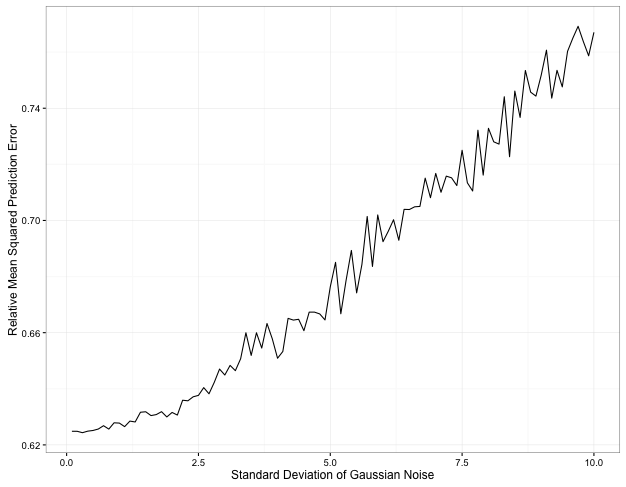
\includegraphics[width=0.75\textwidth]{robust.png}
\caption{\label{fig:robust} Robustness of RMSPE to Noise in Continuois Phenotype}
\end{figure}

\section{Ranking Scores}
Another problem of interest is assigning a score to rank predictions, e.g. given a set of lines of sorghum, and we score the predicted rank orders from some prediction algorithm? The literature is replete with measures of rank ordering. We will focus here two measures of rank ordering correlation, Kendall's Tau and the Normalized Discounted Cumulative Gain. 


\section{Kendall's Tau}

Kendall's Tau is a measure of the correlation between two sets of rankings. Let $Y_1, ..., Y_n$  be a set of observations and let $\hat{Y_1}, ..., \hat{Y_n}$ be a set of predicted observations. Then Any pair of observations $(Y_i, \hat{Y_i})$ and $(Y_j, \hat{Y_j})$, where $i \not= j$, are said to be concordant if the ranks for both elements agree: that is, if both $Y_i > Y_j$ and $\hat{Y_i} > \hat{Y_j}$ or if both $Y_i < Y_j$ and $\hat{Y_i} < \hat{Y_j}$. They are said to be discordant, if $Y_i > Y_j$ and $\hat{Y_i} < \hat{Y_j}$ and $Y_i < Y_j$ and $\hat{Y_i} < \hat{Y_j}$ . If $Y_i = Y_j$ and $\hat{Y_i} = \hat{Y_j}$, the pair is neither concordant nor discordant.

Kendall's Tau is defined as:

\begin{equation}
	\tau = \frac{(number of concordant pairs) - (number of discordant pairs)}{1/2 n(n-1)}
\end{equation}

\subsection{Tables and Figures}



\end{document}


Use the table and tabular commands for basic tables --- see Table~\ref{tab:widgets}, for example. You can upload a figure (JPEG, PNG or PDF) using the files menu. To include it in your document, use the includegraphics command as in the code for Figure~\ref{fig:frog} below.

% Commands to include a figure:
\begin{figure}
\centering
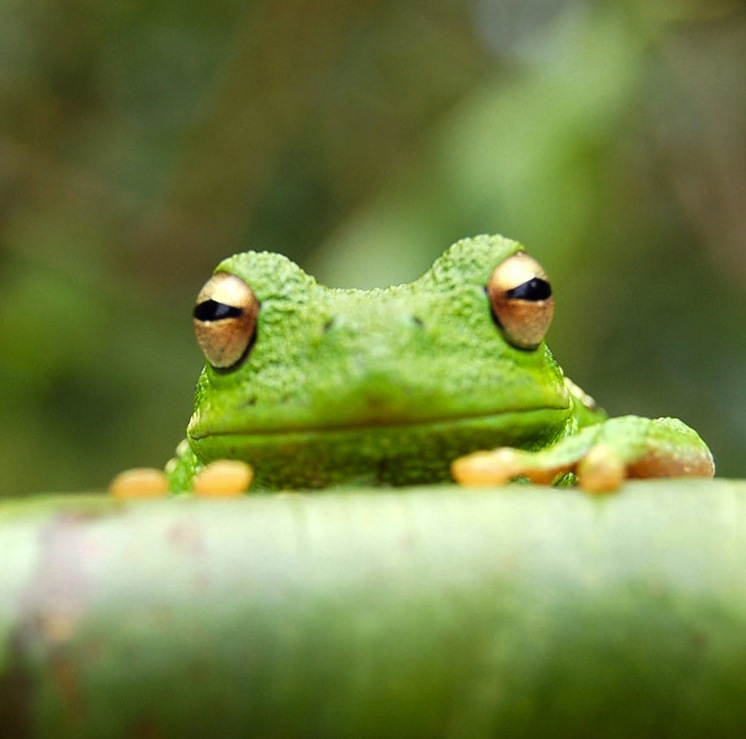
\includegraphics[width=0.5\textwidth]{frog.jpg}
\caption{\label{fig:frog}This is a figure caption.}
\end{figure}

\begin{table}
\centering
\begin{tabular}{l|r}
Item & Quantity \\\hline
Widgets & 42 \\
Gadgets & 13
\end{tabular}
\caption{\label{tab:widgets}An example table.}
\end{table} to your LaTeX file where you want your
% title page.
%
%%%%%%%%%%%%%%%%%%%%%%%%%%%%%%%%%%%%%%%%%
%\title{Title page with logo}
%----------------------------------------------------------------------------------------
%	PACKAGES AND OTHER DOCUMENT CONFIGURATIONS
%----------------------------------------------------------------------------------------

\documentclass[12pt]{article}
\usepackage[english]{babel}
\usepackage[utf8x]{inputenc}
\usepackage{amsmath}
\usepackage{graphicx}
\usepackage[colorinlistoftodos]{todonotes}

\begin{document}

\begin{titlepage}

\newcommand{\HRule}{\rule{\linewidth}{0.5mm}} % Defines a new command for the horizontal lines, change thickness here

\center % Center everything on the page
 
%----------------------------------------------------------------------------------------
%	HEADING SECTIONS
%----------------------------------------------------------------------------------------

\textsc{\LARGE Stat 427 Consulting Project}\\[1.5cm] % Name of your university/college
\textsc{\Large Terraref Prediction Metrics}\\[0.5cm] % Major heading such as course name
\textsc{\large Measures of Prediction and Ranking Accuracy for the TerraRef Project}\\[0.5cm] % Minor heading such as course title

%----------------------------------------------------------------------------------------
%	TITLE SECTION
%----------------------------------------------------------------------------------------

\HRule \\[0.4cm]
{ \huge \bfseries Title}\\[0.4cm] % Title of your document
\HRule \\[1.5cm]
 
%----------------------------------------------------------------------------------------
%	AUTHOR SECTION
%----------------------------------------------------------------------------------------



% If you don't want a supervisor, uncomment the two lines below and remove the section above
\Large \emph{Author:}\\
Kyle \textsc{Payne}\\[3cm] % Your name
Manze \textsc{Qin}\\[3cm] 

%----------------------------------------------------------------------------------------
%	DATE SECTION
%----------------------------------------------------------------------------------------

{\large \today}\\[2cm] % Date, change the \today to a set date if you want to be precise

%----------------------------------------------------------------------------------------
%	LOGO SECTION
%----------------------------------------------------------------------------------------


\includegraphics{logo.png}\\[1cm] % Include a department/university logo - this will require the graphicx package
 
%----------------------------------------------------------------------------------------

\vfill % Fill the rest of the page with whitespace

\end{titlepage}


\begin{abstract}
Your abstract.
\end{abstract}

\section{Introduction}

The following report consists of the Author's Recommendation for Measures of Prediction Quality for the TerraRef Project at the University of Illinois. In this 
preliminary report we will focus on two particular problems that have been addressed so far:

\begin{itemize}
	\item How to determine the accuracy of a continuous prediction on a continous target value (e.g. phenotype).
	\item How to Score Predicted Rankings for some subset of lines (e.g. genotypes).
\end{itemize}

While we only address these problems in a relatively closed sense, the measures that we propose may be applicable to other settings as well. We will define the our measures, describe their respective numerical and statistical properties, make recommendations for using these measures in practice, and produce functions in both the Python and R languages for their implementation. 


\section{Measures}
\label{sec:examples}

\subsection{Continuous Phenotype Prediction}

An example of the types of problems that fall under 'How to determine the accuracy of a continuous prediction on a continous target value (e.g. phenotype)' would be to demonstrate that predicted values are within 20 percent of ground truth values. Thus, we we need a measure that accounts for the difference between the predicted and ground truth (the true observed phenotype values), while also accounting for the \textit{relative degree} by which the predictions are different from the ground truth values. One metric that appears in the literature (citation) is the Relative Mean Squared Prediction Error, or the RMSPE, which we define in equation (*)

Let $Y_1, ..., Y_n$ be a set of ground truth phenotype values, and let $\hat{Y_1}, ..., \hat{Y_n}$ be the set of corresponding predictions for the ground truth phenotype values, then the RMSPE is defined as.

\begin{equation}
	RMSPE = \frac{\sqrt{\sum_{i=1}^{n}(Y_i - \hat{Y_i})^2}}{\sqrt{\sum_{i=1}^{n}Y_i^2}}}
\end{equation}

The square of the numerator $\sum_{i=1}^{n}(Y_i - \hat{Y_i})^2$ is a well-studied function within the machine learning and statistics community, known as the Mean Squared Prediction Error, or (MSPE). This is an easily computed, and numerically stable quantity that provides several desirable large sample properties. The denominator of $RMSPE$ can be viewed as the difference of the continuous ground-truth phenotype values from $0$. Thus, $RMSPE$ acts a relative measure of the difference between the ground truth continuous phenotype values, expressed in units of the continuous phenotype. Using this measure, an experimenter could make a statment such as, "I demonstrated that the predicted values are within $0.2$ of the ground truth values". This type of measure could be helpful for determining prediction accuracy for both Terminal Biomass and 3D Structural Models. Moreover, the $RMSPE$ could also be used to compare the prediction accuracy between competing models, such as comparing algorithm predictions v.s. the Lemnatec Software. 

\subsection*{Examples}

If a prediction model produces a set of predictions $\hat{Y_1}, ..., \hat{Y_n}$, for a set of ground truth continuous phenotype values $Y_1, ..., Y_n$, then 
let's state that 

\begin{equation}
	RMSPE \leq 0.20 \Rightarrow \sqrt{\sum_{i=1}^{n}(Y_i - \hat{Y_i})^2} \leq 0.2\sqrt{\sum_{i=1}^{n}Y_i^2}}
\end{equation}

The equation above describes the case where the $RMSPE$ being less than or equal to 20 percent is equivalent to stating that the mean squared prediction error is bounded by $0.2$ the size of the ground truth phenotype values. The quantity on the left-hand side of the inequality is an example of a commonly used measure of distance in mathematics, engineering, statistics, computer science, etc. known as the \textit{Norm} (Weisstein, Eric W. "Norm." From MathWorld--A Wolfram Web Resource. http://mathworld.wolfram.com/Norm.html).

Let $RMSPE_L$ be the relative mean squared prediction error of Lemnatec software predictions on the ground truth continuous phenotype values $Y_1, ..., Y_n$, which we will denote as $Y_1^{*}, ..., Y_n^{*}$. Let $RMSPE_M$ be the relative mean squared prediction error of some prediction model or algorithm. Then, making a determination such as 'algorithm predictions are no less accurate than values predicted via LemnaTec software', would require comparing $RMSPE_L$ and $RMSPE_M$, thus

\begin{equation}
	$RMSPE_M$ \leq $RMSPE_L$ 
\end{equation}

Let's assume that the predictions are for the same set of ground truth continuous phenotype values $Y_1, ..., Y_n$, then the preceding equation is 
equivalent to 

\begin{equation}
	$RMSPE_M$ \leq $RMSPE_L$ \Rightarrow \frac{\sqrt{\sum_{i=1}^{n}(Y_i - \hat{Y_i})^2}}{\sqrt{\sum_{i=1}^{n}Y_i^2}}} \leq \frac{\sqrt{\sum_{i=1}^{n}(Y_i - Y_i^{*})^2}}{\sqrt{\sum_{i=1}^{n}Y_i^2}}} \Rightarrow \sum_{i=1}^{n}(Y_i - \hat{Y_i})^2 \leq \sum_{i=1}^{n}(Y_i - Y_i^{*})^2
\end{equation}

Thus, if we compare two prediction models in $RMSPE$ on the same set of data, the comparision is equivalent to just comparing the average squared difference between the predictions and the ground truth values.
\subsection{Performance}
The Relative Mean Squared Prediction Error Performs well in situations in which there is additional noise in the continuous phenotype values $Y_1, ..., Y_n$.
For the following example, let's assume that some prediction algorithm has been fitted to a set of training data. In this case, we chose a Random Forest Model to predict Stem Biomass using the plot identifier and the precipitation data on a sub-sample of simulated data. We trained the random forest model on a sub-sample of simulated data. Predictions were then made using a test sample of the data, with additional mean $0$ gaussian random noise applied to the Stem Biomass data. The RMSPE measure increases like a polynomial with increasingly variable noise. However, the RMSPE remains relatively robust to deviations from the true Prediction Error, and only increases to very large values as the 

\begin{figure}
\centering
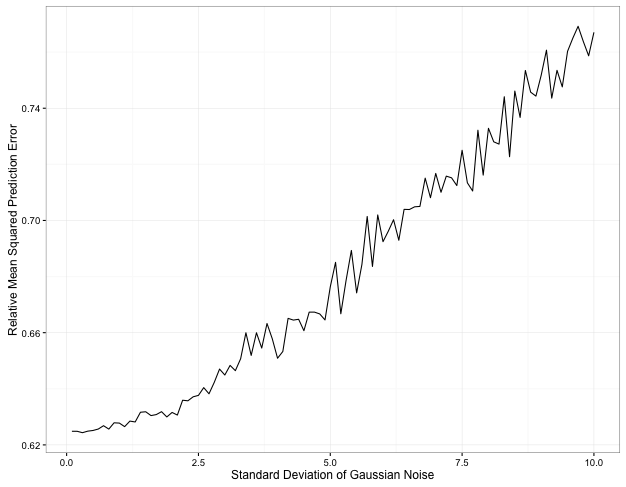
\includegraphics[width=0.75\textwidth]{robust.png}
\caption{\label{fig:robust} Robustness of RMSPE to Noise in Continuois Phenotype}
\end{figure}

\section{Ranking Scores}
Another problem of interest is assigning a score to rank predictions, e.g. given a set of lines of sorghum, and we score the predicted rank orders from some prediction algorithm? The literature is replete with measures of rank ordering. We will focus here two measures of rank ordering correlation, Kendall's Tau and the Normalized Discounted Cumulative Gain. 


\section{Kendall's Tau}

Kendall's Tau is a measure of the correlation between two sets of rankings. Let $Y_1, ..., Y_n$  be a set of observations and let $\hat{Y_1}, ..., \hat{Y_n}$ be a set of predicted observations. Then Any pair of observations $(Y_i, \hat{Y_i})$ and $(Y_j, \hat{Y_j})$, where $i \not= j$, are said to be concordant if the ranks for both elements agree: that is, if both $Y_i > Y_j$ and $\hat{Y_i} > \hat{Y_j}$ or if both $Y_i < Y_j$ and $\hat{Y_i} < \hat{Y_j}$. They are said to be discordant, if $Y_i > Y_j$ and $\hat{Y_i} < \hat{Y_j}$ and $Y_i < Y_j$ and $\hat{Y_i} < \hat{Y_j}$ . If $Y_i = Y_j$ and $\hat{Y_i} = \hat{Y_j}$, the pair is neither concordant nor discordant.

Kendall's Tau is defined as:

\begin{equation}
	\tau = \frac{(number of concordant pairs) - (number of discordant pairs)}{1/2 n(n-1)}
\end{equation}

\subsection{Tables and Figures}



\end{document}


Use the table and tabular commands for basic tables --- see Table~\ref{tab:widgets}, for example. You can upload a figure (JPEG, PNG or PDF) using the files menu. To include it in your document, use the includegraphics command as in the code for Figure~\ref{fig:frog} below.

% Commands to include a figure:
\begin{figure}
\centering
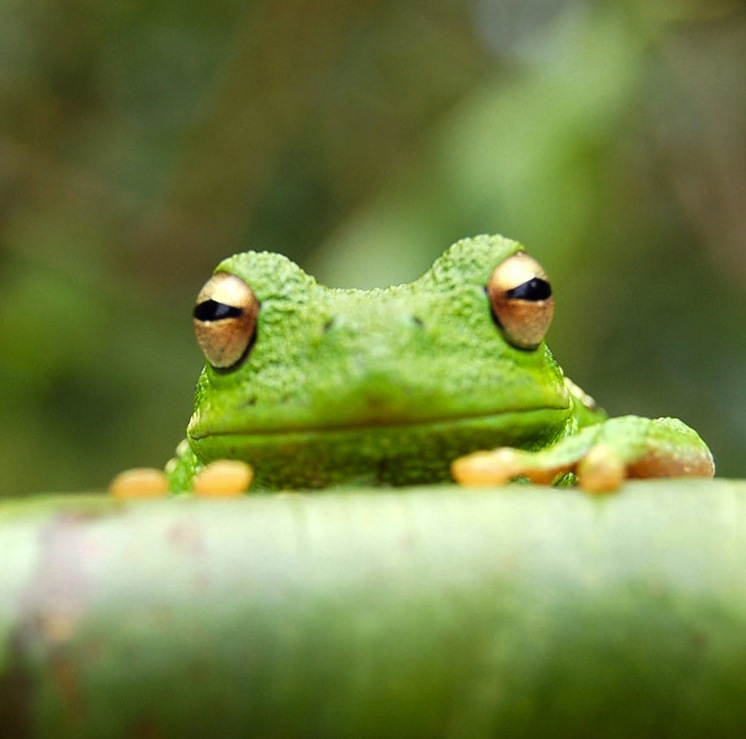
\includegraphics[width=0.5\textwidth]{frog.jpg}
\caption{\label{fig:frog}This is a figure caption.}
\end{figure}

\begin{table}
\centering
\begin{tabular}{l|r}
Item & Quantity \\\hline
Widgets & 42 \\
Gadgets & 13
\end{tabular}
\caption{\label{tab:widgets}An example table.}
\end{table} to your LaTeX file where you want your
% title page.
%
%%%%%%%%%%%%%%%%%%%%%%%%%%%%%%%%%%%%%%%%%
%\title{Title page with logo}
%----------------------------------------------------------------------------------------
%	PACKAGES AND OTHER DOCUMENT CONFIGURATIONS
%----------------------------------------------------------------------------------------

\documentclass[12pt]{article}
\usepackage[english]{babel}
\usepackage[utf8x]{inputenc}
\usepackage{amsmath}
\usepackage{graphicx}
\usepackage[colorinlistoftodos]{todonotes}

\begin{document}

\begin{titlepage}

\newcommand{\HRule}{\rule{\linewidth}{0.5mm}} % Defines a new command for the horizontal lines, change thickness here

\center % Center everything on the page
 
%----------------------------------------------------------------------------------------
%	HEADING SECTIONS
%----------------------------------------------------------------------------------------

\textsc{\LARGE Stat 427 Consulting Project}\\[1.5cm] % Name of your university/college
\textsc{\Large Terraref Prediction Metrics}\\[0.5cm] % Major heading such as course name
\textsc{\large Measures of Prediction and Ranking Accuracy for the TerraRef Project}\\[0.5cm] % Minor heading such as course title

%----------------------------------------------------------------------------------------
%	TITLE SECTION
%----------------------------------------------------------------------------------------

\HRule \\[0.4cm]
{ \huge \bfseries Title}\\[0.4cm] % Title of your document
\HRule \\[1.5cm]
 
%----------------------------------------------------------------------------------------
%	AUTHOR SECTION
%----------------------------------------------------------------------------------------



% If you don't want a supervisor, uncomment the two lines below and remove the section above
\Large \emph{Author:}\\
Kyle \textsc{Payne}, Manze \textsc{Qin}, Tangwei Li  % Your name
\\[3cm] 

%----------------------------------------------------------------------------------------
%	DATE SECTION
%----------------------------------------------------------------------------------------

{\large \today}\\[2cm] % Date, change the \today to a set date if you want to be precise

%----------------------------------------------------------------------------------------
%	LOGO SECTION
%----------------------------------------------------------------------------------------

% \
\includegraphics{UIUC_seal.png}[scale=0.1]\\[1cm] % Include a department/university logo - this will require the graphicx package
 
%----------------------------------------------------------------------------------------

\vfill % Fill the rest of the page with whitespace

\end{titlepage}

\section{Introduction}

The following report consists of the Author's Recommendation for Measures of Prediction Quality for the TerraRef Project at the University of Illinois. In this 
preliminary report we will focus on two particular problems that have been addressed so far:

\begin{itemize}
	\item How to determine the accuracy of a continuous prediction on a continous target value (e.g. phenotype).
	\item How to Score Predicted Rankings for some subset of lines (e.g. genotypes).
\end{itemize}

While we only address these problems in a relatively closed sense, the measures that we propose may be applicable to other settings as well. We will define the our measures, describe their respective numerical and statistical properties, make recommendations for using these measures in practice, and produce functions in both the Python and R languages for their implementation. 


\section{Measures}
\label{sec:examples}

\subsection{Continuous Phenotype Prediction}

An example of the types of problems that fall under 'How to determine the accuracy of a continuous prediction on a continous target value (e.g. phenotype)' would be to demonstrate that predicted values are within 20 percent of ground truth values. Thus, we we need a measure that accounts for the difference between the predicted and ground truth (the true observed phenotype values), while also accounting for the \textit{relative degree} by which the predictions are different from the ground truth values. One metric that appears in the literature (citation) is the Relative Mean Squared Prediction Error, or the RMSPE, which we define in equation (*)

Let $Y_1, ..., Y_n$ be a set of ground truth phenotype values, and let $\hat{Y_1}, ..., \hat{Y_n}$ be the set of corresponding predictions for the ground truth phenotype values, then the RMSPE is defined as.

\begin{equation}
	RMSPE = \frac{\sqrt{\sum_{i=1}^{n}(Y_i - \hat{Y_i})^2}}{\sqrt{\sum_{i=1}^{n}Y_i^2}}}
\end{equation}

The square of the numerator $\sum_{i=1}^{n}(Y_i - \hat{Y_i})^2$ is a well-studied function within the machine learning and statistics community, known as the Mean Squared Prediction Error, or (MSPE). This is an easily computed, and numerically stable quantity that provides several desirable large sample properties. The denominator of $RMSPE$ can be viewed as the difference of the continuous ground-truth phenotype values from $0$. Thus, $RMSPE$ acts a relative measure of the difference between the ground truth continuous phenotype values, expressed in units of the continuous phenotype. Using this measure, an experimenter could make a statment such as, "I demonstrated that the predicted values are within $0.2$ of the ground truth values". This type of measure could be helpful for determining prediction accuracy for both Terminal Biomass and 3D Structural Models. Moreover, the $RMSPE$ could also be used to compare the prediction accuracy between competing models, such as comparing algorithm predictions v.s. the Lemnatec Software. 

\subsection*{Examples}

If a prediction model produces a set of predictions $\hat{Y_1}, ..., \hat{Y_n}$, for a set of ground truth continuous phenotype values $Y_1, ..., Y_n$, then 
let's state that 

\begin{equation}
	RMSPE \leq 0.20 \Rightarrow \sqrt{\sum_{i=1}^{n}(Y_i - \hat{Y_i})^2} \leq 0.2\sqrt{\sum_{i=1}^{n}Y_i^2}}
\end{equation}

The equation above describes the case where the $RMSPE$ being less than or equal to 20 percent is equivalent to stating that the mean squared prediction error is bounded by $0.2$ the size of the ground truth phenotype values. The quantity on the left-hand side of the inequality is an example of a commonly used measure of distance in mathematics, engineering, statistics, computer science, etc. known as the \textit{Norm} (Weisstein, Eric W. "Norm." From MathWorld--A Wolfram Web Resource. http://mathworld.wolfram.com/Norm.html).

Let $RMSPE_L$ be the relative mean squared prediction error of Lemnatec software predictions on the ground truth continuous phenotype values $Y_1, ..., Y_n$, which we will denote as $Y_1^{*}, ..., Y_n^{*}$. Let $RMSPE_M$ be the relative mean squared prediction error of some prediction model or algorithm. Then, making a determination such as 'algorithm predictions are no less accurate than values predicted via LemnaTec software', would require comparing $RMSPE_L$ and $RMSPE_M$, thus

\begin{equation}
	$RMSPE_M$ \leq $RMSPE_L$ 
\end{equation}

Let's assume that the predictions are for the same set of ground truth continuous phenotype values $Y_1, ..., Y_n$, then the preceding equation is 
equivalent to 

\begin{equation}
	$RMSPE_M$ \leq $RMSPE_L$ \Rightarrow \frac{\sqrt{\sum_{i=1}^{n}(Y_i - \hat{Y_i})^2}}{\sqrt{\sum_{i=1}^{n}Y_i^2}}} \leq \frac{\sqrt{\sum_{i=1}^{n}(Y_i - Y_i^{*})^2}}{\sqrt{\sum_{i=1}^{n}Y_i^2}}} \Rightarrow \sum_{i=1}^{n}(Y_i - \hat{Y_i})^2 \leq \sum_{i=1}^{n}(Y_i - Y_i^{*})^2
\end{equation}

Thus, if we compare two prediction models in $RMSPE$ on the same set of data, the comparision is equivalent to just comparing the average squared difference between the predictions and the ground truth values.
\subsection{Performance}
The Relative Mean Squared Prediction Error Performs well in situations in which there is additional noise in the continuous phenotype values $Y_1, ..., Y_n$.
For the following example, let's assume that some prediction algorithm has been fitted to a set of training data. In this case, we chose a Random Forest Model to predict Stem Biomass using the plot identifier and the precipitation data on a sub-sample of simulated data. We trained the random forest model on a sub-sample of simulated data. Predictions were then made using a test sample of the data, with additional mean $0$ gaussian random noise applied to the Stem Biomass data. The RMSPE measure increases like a polynomial with increasingly variable noise. However, the RMSPE remains relatively robust to deviations from the true Prediction Error, and only increases to very large values as the 

\begin{figure}
\centering
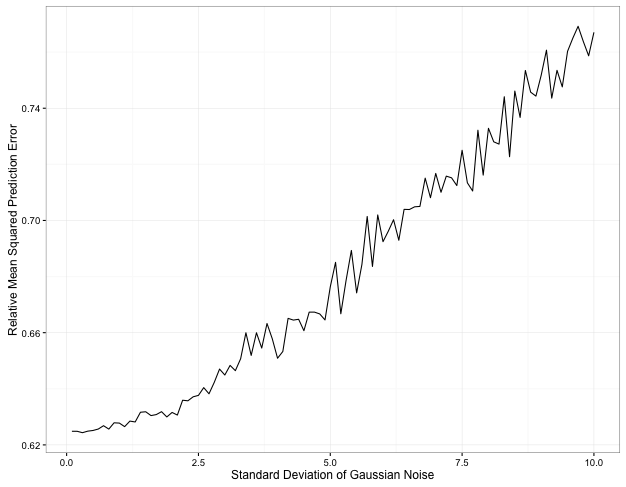
\includegraphics[width=0.75\textwidth]{robust.png}
\caption{\label{fig:robust} Robustness of RMSPE to Noise in Continuois Phenotype}
\end{figure}

\section{Ranking Scores}
Another problem of interest is assigning a score to rank predictions, e.g. given a set of lines of sorghum, and we score the predicted rank orders from some prediction algorithm? The literature is replete with measures of rank ordering. We will focus here two measures of rank ordering correlation, Kendall's Tau and the Normalized Discounted Cumulative Gain. 


\subsection{Kendall's Tau}

Kendall's Tau is a measure of the correlation between two sets of rankings. Let $Y_1, ..., Y_n$  be a set of observations and let $\hat{Y_1}, ..., \hat{Y_n}$ be a set of predicted observations. Then Any pair of observations $(Y_i, \hat{Y_i})$ and $(Y_j, \hat{Y_j})$, where $i \not= j$, are said to be concordant if the ranks for both elements agree: that is, if both $Y_i > Y_j$ and $\hat{Y_i} > \hat{Y_j}$ or if both $Y_i < Y_j$ and $\hat{Y_i} < \hat{Y_j}$. They are said to be discordant, if $Y_i > Y_j$ and $\hat{Y_i} < \hat{Y_j}$ and $Y_i < Y_j$ and $\hat{Y_i} < \hat{Y_j}$ . If $Y_i = Y_j$ and $\hat{Y_i} = \hat{Y_j}$, the pair is neither concordant nor discordant.

Kendall's Tau is defined as:

\begin{equation}
	\tau = \frac{(\text{number of concordant pairs}) - (\text{number of discordant pairs)}}{1/2 n(n-1)}
\end{equation}

If both sets, the ground truth and predicted values are completely concordant in rank, then $\tau = 1$. Likewise, if both sets are in perfect disagreement, then 
$\tau = -1$. Kendall's Tau is analogous to a correlation coefficient in this manner. While Kendall's $\tau$ is easy to interprete, $\tau$ does not weight discordance differently depending on where in the rankings the discordance occurs. Therefore, one may be interested in a different ranking score, which we describe below.


\subsection{Normalized Discounted Cumulative Gain}





\end{document}


Use the table and tabular commands for basic tables --- see Table~\ref{tab:widgets}, for example. You can upload a figure (JPEG, PNG or PDF) using the files menu. To include it in your document, use the includegraphics command as in the code for Figure~\ref{fig:frog} below.

% Commands to include a figure:
\begin{figure}
\centering
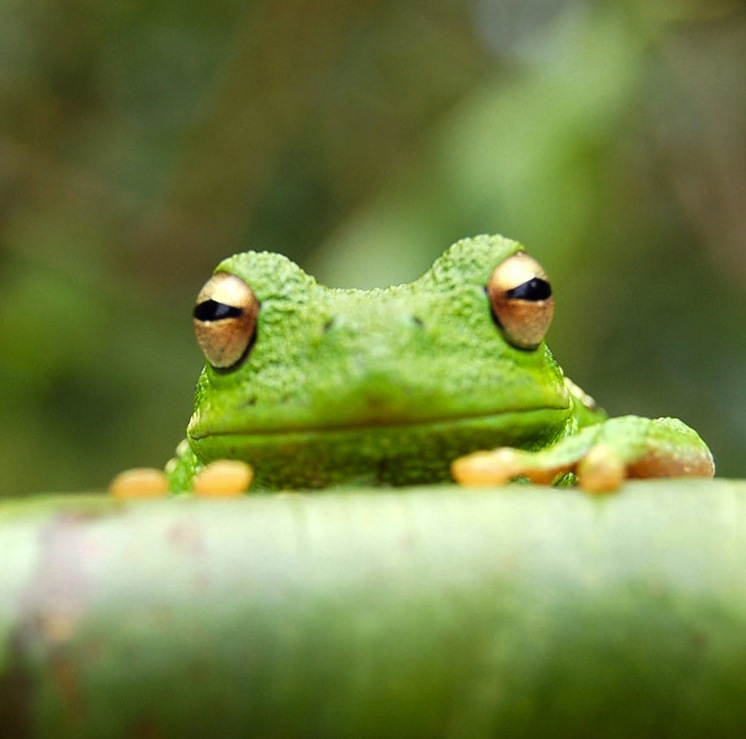
\includegraphics[width=0.5\textwidth]{frog.jpg}
\caption{\label{fig:frog}This is a figure caption.}
\end{figure}

\begin{table}
\centering
\begin{tabular}{l|r}
Item & Quantity \\\hline
Widgets & 42 \\
Gadgets & 13
\end{tabular}
\caption{\label{tab:widgets}An example table.}
\end{table}